\documentclass[10pt]{beamer}

\usetheme{metropolis}

\usepackage{graphicx}
\usepackage{siunitx}
\usepackage{amsmath}
\usepackage{physics}
\usepackage[labelformat=empty]{caption}
\newtheorem{mydef}{Definition}
\setbeamertemplate{itemize subitem}[square]

\title{Philosophically Consistent Gravitational-Wave Background Searches}
\author{Duncan Wilkie}
\date{2 December 2022}

\begin{document}

\begin{frame}
  \titlepage
\end{frame}

\begin{frame}
  % What the paper is
  \frametitle{Paper}
  \begin{center}
    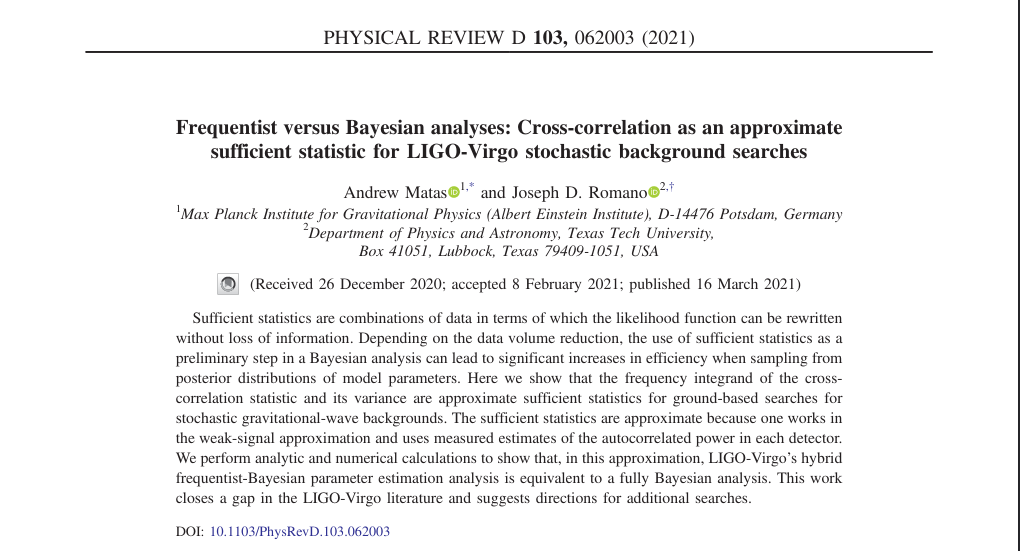
\includegraphics[scale=0.3]{abstract.png}
  \end{center}
\end{frame}

\begin{frame}
  % Terms requiring explanation
  \frametitle{Paper}
  \begin{figure}
    \centering
    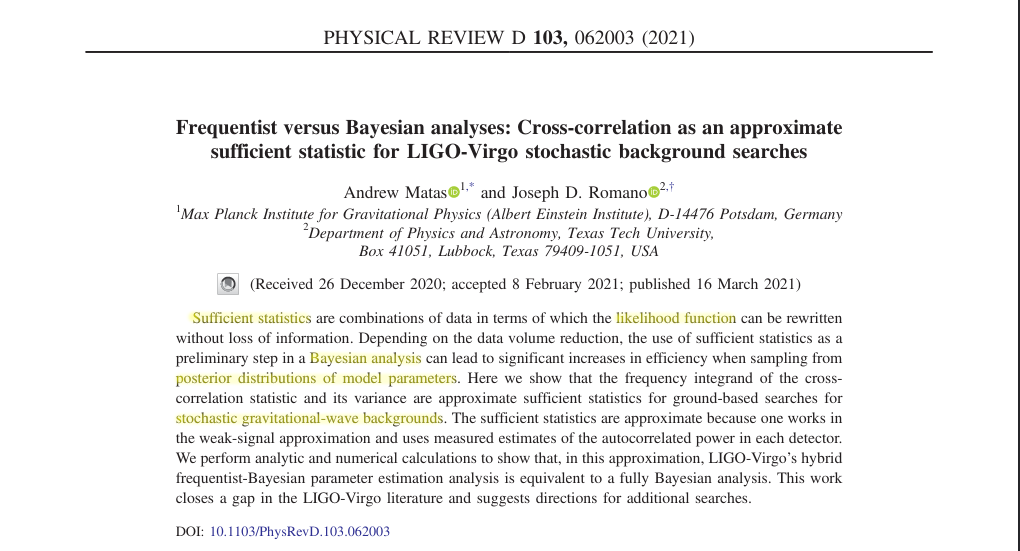
\includegraphics[scale=0.3]{abstract_interesting.png}
  \end{figure}
\end{frame}

\begin{frame}
  \frametitle{Stochastic Backgrounds?}
  \begin{itemize}
  \item LIGO is optimized for transients.
  \item Stochastic $\Rightarrow$ ``random stuff accumulating''
  \item Background $\Rightarrow$ ``isotropic''
  \end{itemize}
  \begin{figure}
      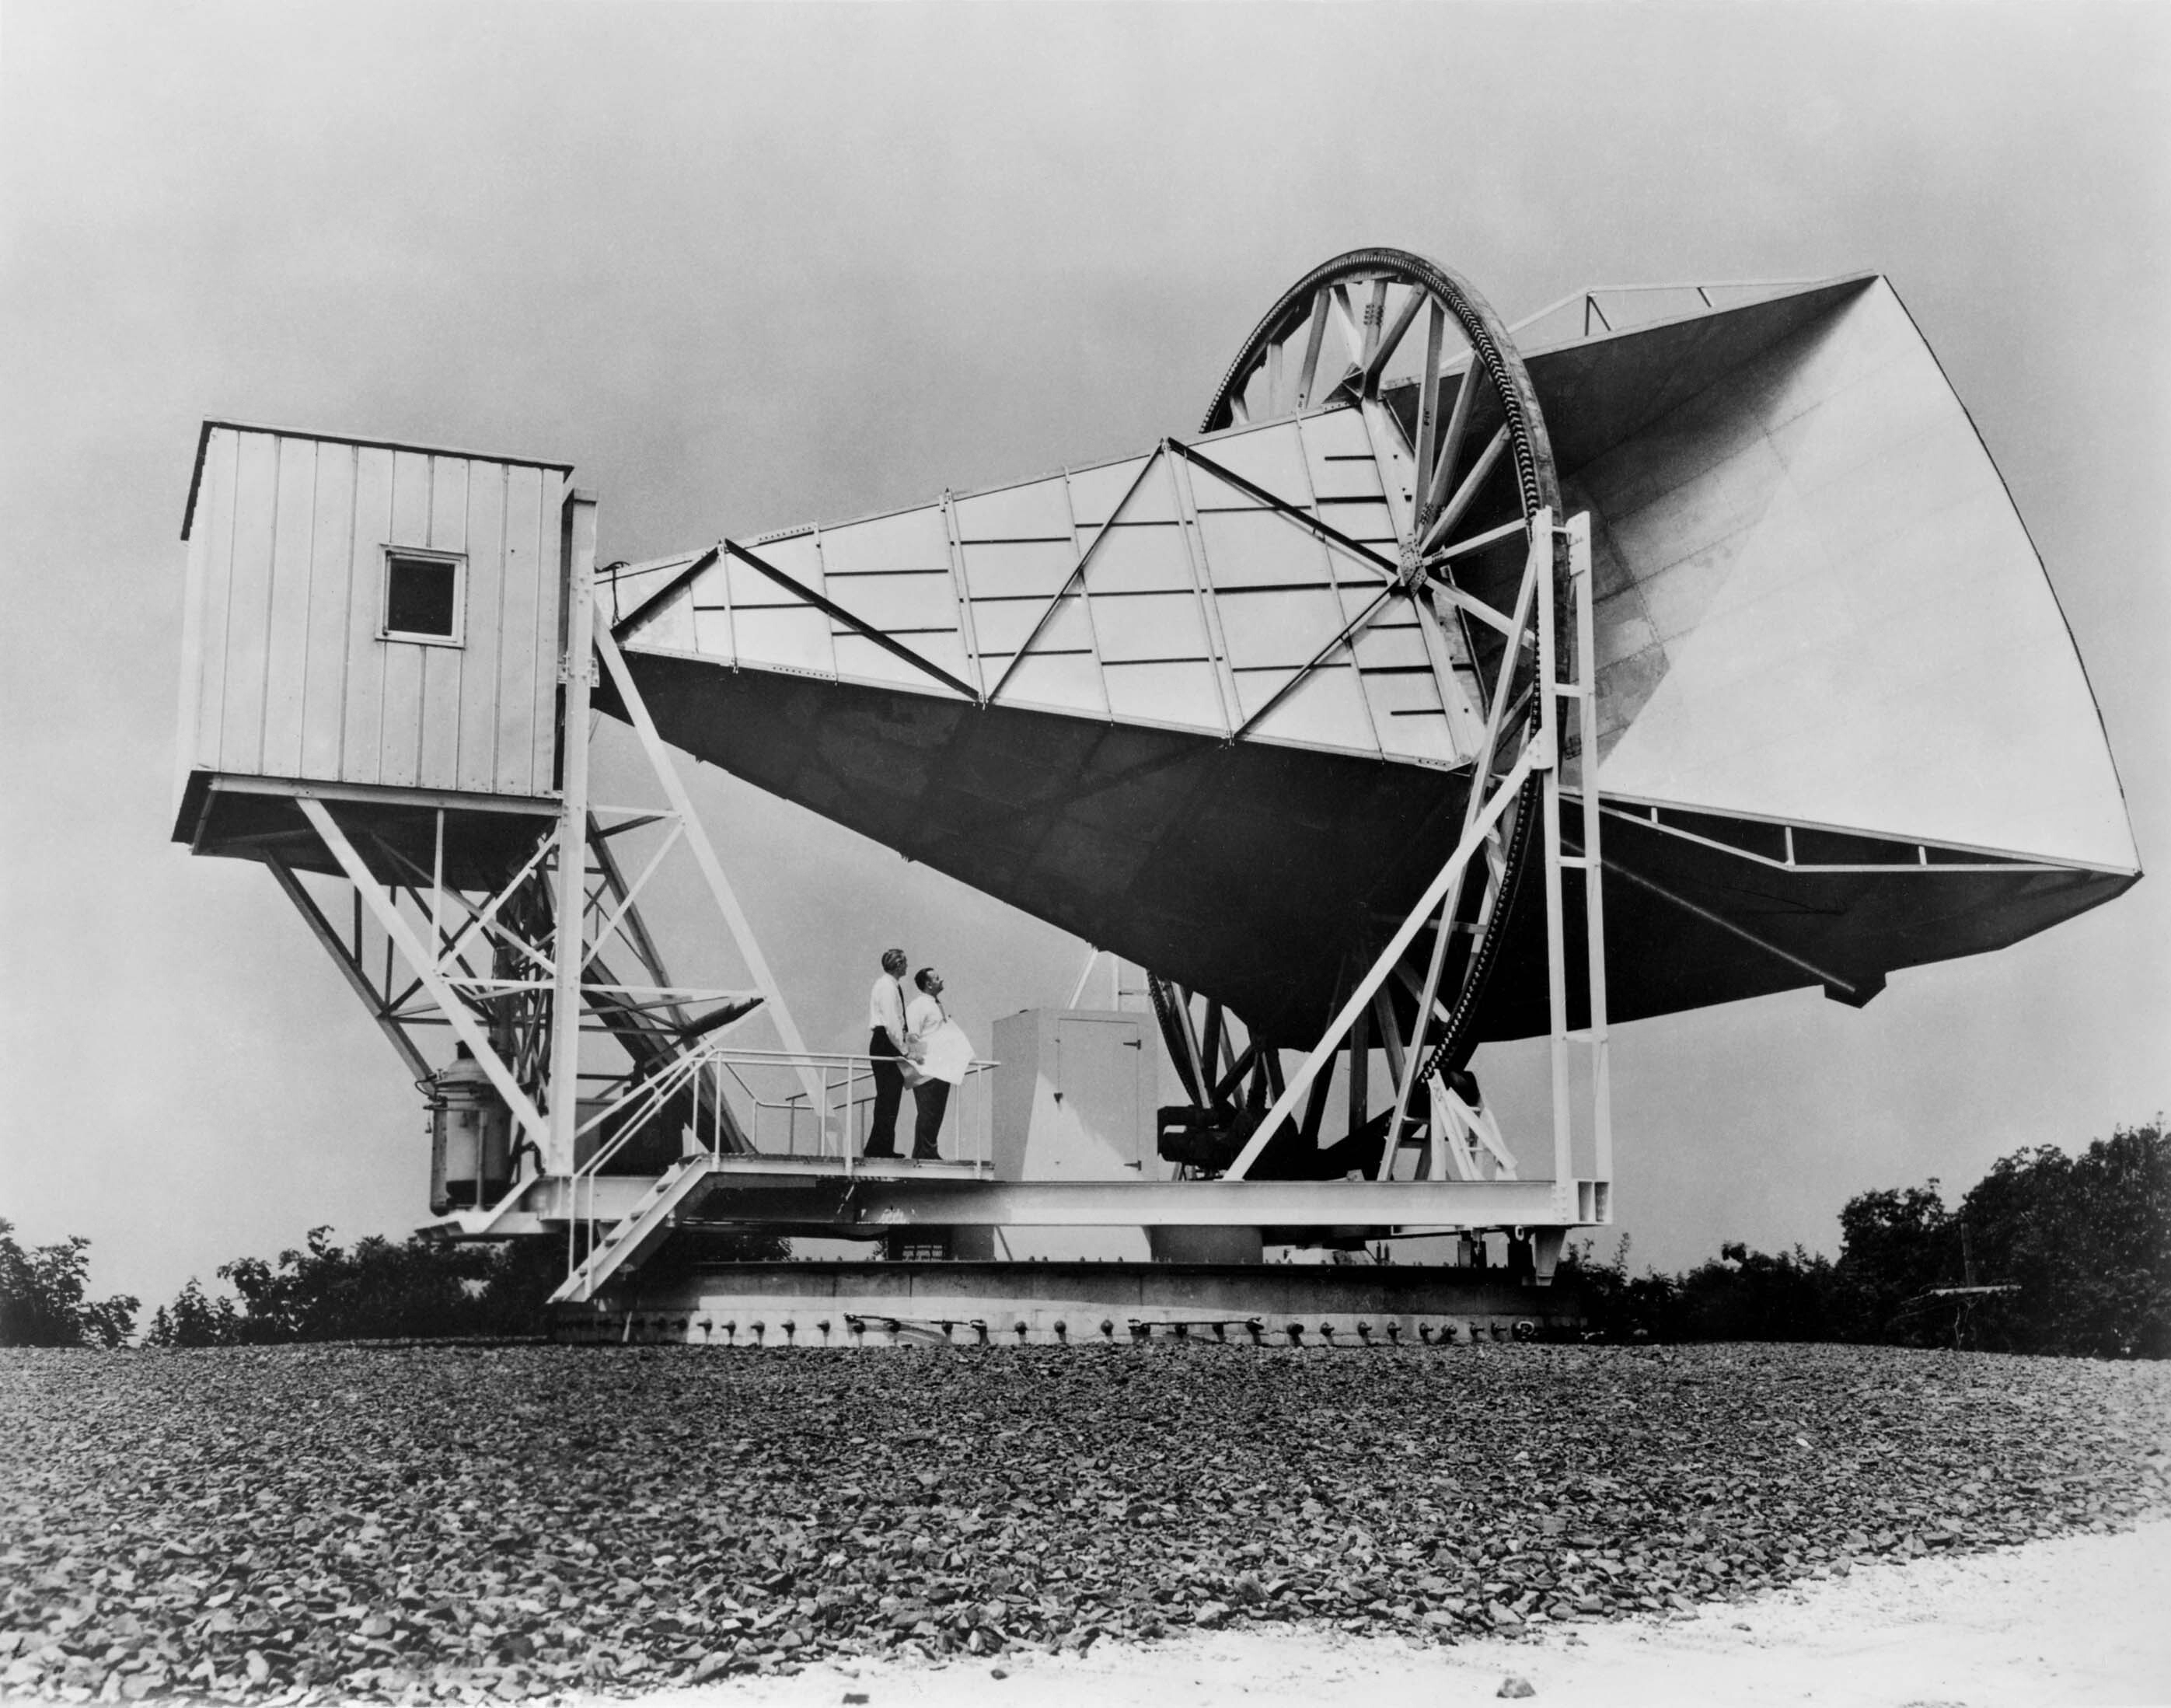
\includegraphics[scale=0.15]{detector.jpg}
      \caption{Idiopathic ``noise'' in this}
      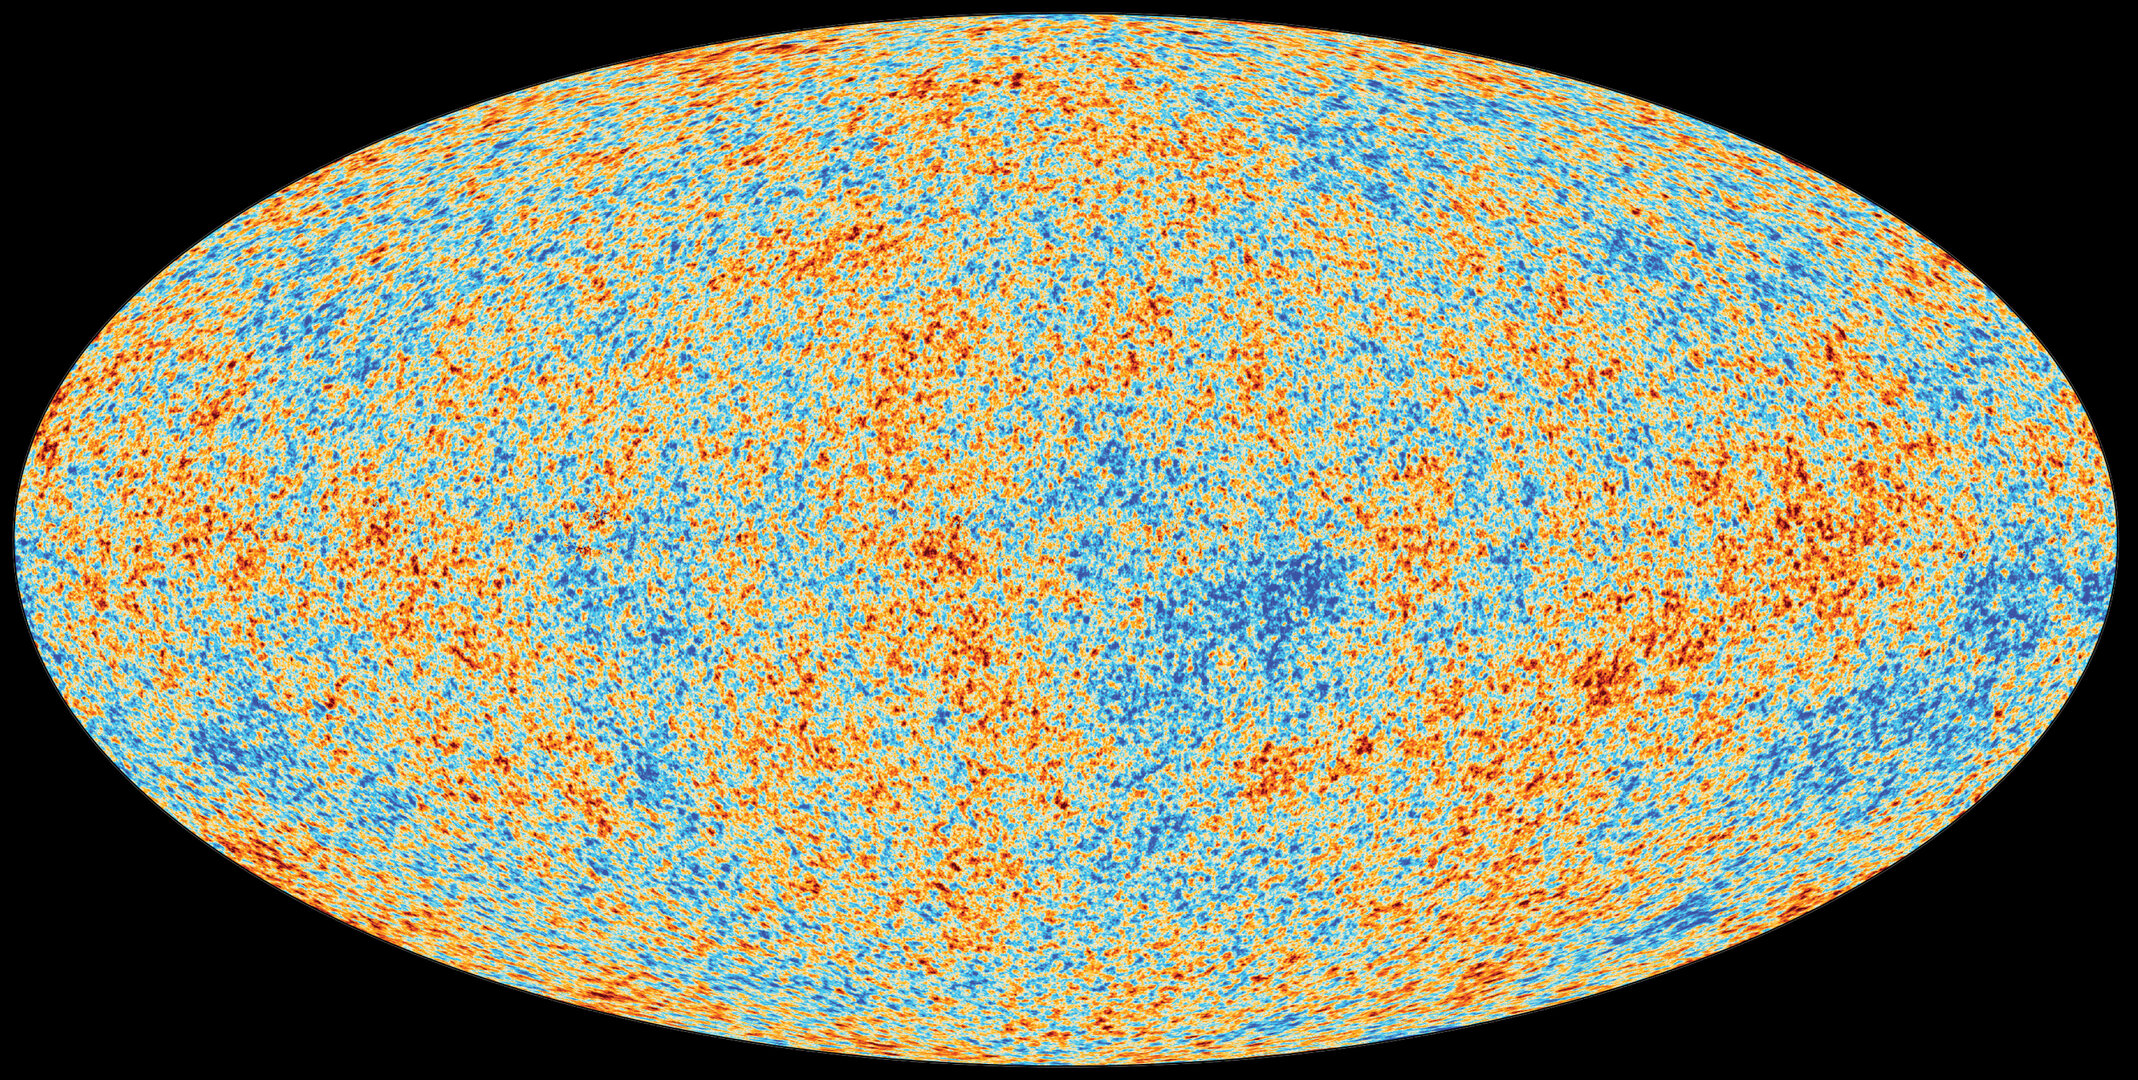
\includegraphics[scale=0.05]{cmb.jpg}
      \caption{Was this}
  \end{figure}
  % Just as statistical properties of the CMB are a wealth of cosmological information (anisotropy),
  % so too might those of the GWSB.
\end{frame}

\begin{frame}
  \frametitle{Stochastic Backgrounds?}
  What unresolved astrophysical events might accumulate to appear as detector noise?
  \begin{itemize}
  \item Inflation
  \item Singular points where cosmic strings/superstrings intersect
  \item Discontinuous phase transitions in the early universe
    \begin{itemize}
    \item Strong-force disunity
    \item Electroweak baryogenesis
    \item Plasma bubble collisions and attendant shock waves
    \item Magnetohydrodynamics
    \item Most of the alternative electroweak models
    \end{itemize}
  \item Pre-Bang stuff
  \item Lots of weak BBHs/BNSs
  \item Close compact binaries (e.g. two orbiting white dwarfs in our galaxy)
  \item Supernovae
  \item Pulsars/Magnetars
  \item Big Bang itself

  \end{itemize}
\end{frame}
\begin{frame}
  \frametitle{Stochastic Backgrounds?}
  \begin{figure}
    \centering
    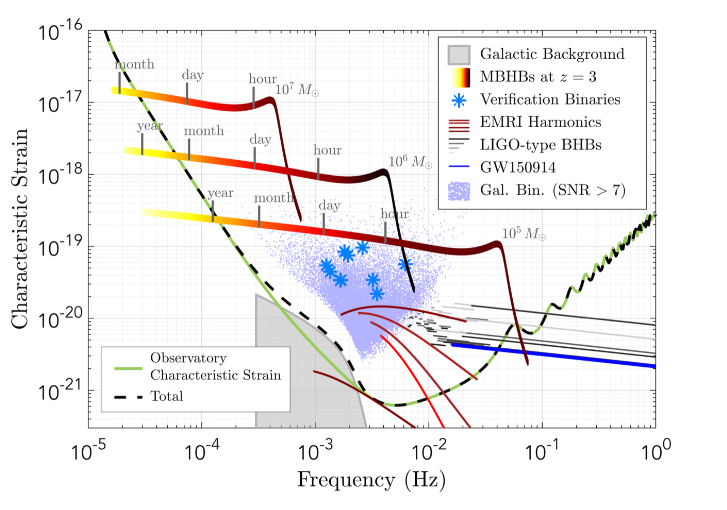
\includegraphics[scale=0.3]{noise?.png}
    \caption*{Mostly at low frequency, so we need LISA (Nelson Christensen 2019 Rep. Prog. Phys. 82 016903)}
  \end{figure}
\end{frame}

\begin{frame}
  \frametitle{Stochastic Backgrounds?}
  \begin{itemize}
  \item This has been looked for in LIGO! (maybe the effect is massive)
  \item Nothing found...
  \item Established a technique though!
  \item This paper justifies the current hybrid technique from a Bayesian perspective.
  \end{itemize}
\end{frame}

\begin{frame}
  \frametitle{What's the Problem?}
  The current method:
  \begin{enumerate}
  \item Calculate a frequentist statistic (frequency-totaled detector X-correlation and its variance) over small time bins,
  \item Weight per unit noise, and
  \item Feed this into Bayesian analysis that checks for correlated noise attributable to background.
  \end{enumerate}
  This is concerning \textit{prima facie}; probabilities mean \textit{completely} different things for the two schools!
  It's not bad as it looks, because you can ask each approach what it thinks of the other, but it's still ugly.

  Frequentist methods tend to have poor algorithmics too...much of the recent boom in Bayesianism is likely attributable to MCMC!
\end{frame}

\begin{frame}
  \frametitle{What's the Problem?}
  Many think the Bayesian philosophy is just \textit{right,} too.
  \begin{itemize}
  \item Frequentist statistics $\longleftrightarrow$ objective characteristics of repeated, well-defined random experiments,
    but QM means repeated experiments are \textit{purely imaginary.}
  \item What about deterministic phenomena that are too hard to compute?
  \item Bayesian statistics $\longleftrightarrow$ scientific reasoning.
  \item Bayesian statistics $\longleftrightarrow$ inductive reasoning (+ transitive corollary).
  \item Minimizes nuisance variables (frequentists can't even see them).
  \item Frequentism is hard to get right (Bertrand's paradoxes; measure theory is an error unto itself; ``The Null Ritual'').
  \item Frequentism is just less powerful (cf. constructive vs classical logic);
  \item Very Platonic (clean line between objects and their shadows).
  \item Notable involvement from physicists! (Cox, Jeffreys, Jaynes).
  \end{itemize}
  Counterclaims: ``What the heck is the Born rule then?'' ``Priors are hard to decide.''
\end{frame}

\begin{frame}
  \frametitle{The Bayesian Process}
  The fundamental inferential principle is Bayes' theorem:
  \[
    P(H \mid E) = \frac{P(E \mid H) \cdot P(H)}{P(E)},
  \]
  \[
    \text{Posterior} = \frac{\text{Likelihood} \cdot \text{Prior}}{\text{Evidence}},
  \]
  or ``the probability of a hypothesis given some new evidence is the probability of the evidence, given the hypothesis,
  times the probability of the hypothesis before the new evidence, divided by the probability of the evidence before it was observed.''

  This paper proves that, to an approximation, a current frequentist statistic losslessly compresses the information in the likelihood function,
  meaning the method is correct from a Bayesian perspective.
\end{frame}

\begin{frame}
  \frametitle{The Bayesian Process}
  The simplest sufficient statistic: the sample mean for a constant signal in standardized Gaussian noise of known variance, $d_{i} = a + n_{i}$.
  For $N$ data points, the likelihood of a datum $d$ is
  \[
    p(d \mid a) = \frac{1}{(2\pi)^{N/2}\sigma^{N}}\exp\qty[-\frac{1}{2\sigma^{2}}\sum_{i}(d_{i} - a)^{2}]
  \]
  The average of the $d_{i}$, $\hat{a}$, is an unbiased, maximum-likelihood estimator; applying a little identity,
  \[
    p(d \mid a) = \frac{1}{(2\pi)^{N/2}\sigma^{N}}\exp\qty[-\frac{1}{2\sigma^{2}}\sum_{i}d_{i}^{2}]\exp\qty[\frac{\hat{a}^{2}}{2\sigma^{2}_{\hat{a}}}]
    \exp\qty[-\frac{(\hat{a} - a)^{2}}{2\sigma_{\hat{a}}^{2}}]
  \]
  Sufficiency of the statistic $\hat{a}$ $\longleftrightarrow$ likelihood $=f(\text{anything but } a)g(\hat{a})$.
\end{frame}

\begin{frame}
  \frametitle{The Result}
  \begin{itemize}
  \item The paper does an analysis for a strong, white signal and a colored, but weak signal.
  \item The former result is just a weaker, illustrative result, so we can look at the latter.
  \item A result for arbitrarily large signals is proved in an appendix, but it's not manifestly different.
  \end{itemize}
\end{frame}

\begin{frame}
  \frametitle{The Result}
  \begin{figure}
    \centering

    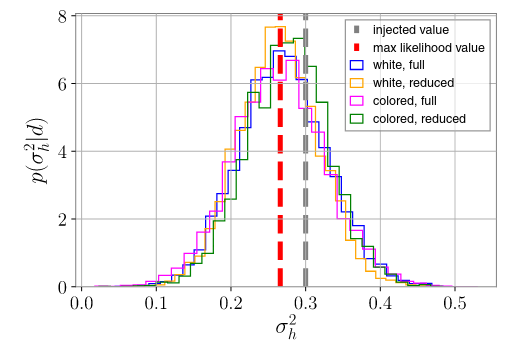
\includegraphics[scale=.5]{fig2p.png}
    \caption{Fig 2}
  \end{figure}
\end{frame}

\begin{frame}
  \frametitle{The Result}
  \begin{figure}
    \centering
    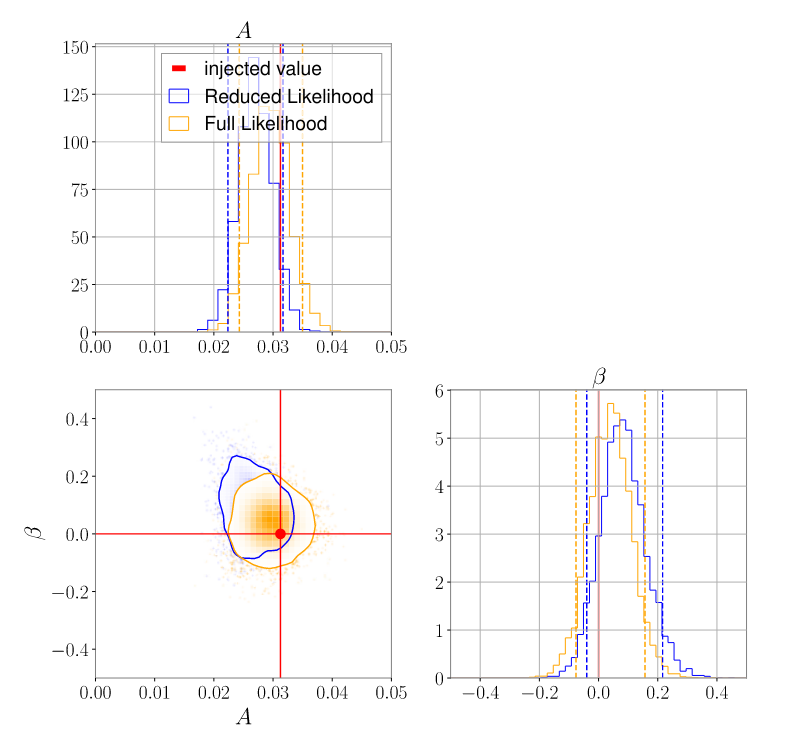
\includegraphics[scale=.29]{fig3p.png}
    \caption{Fig 3}
  \end{figure}
\end{frame}

\begin{frame}
  \frametitle{The Result}
  \begin{figure}
    \centering
    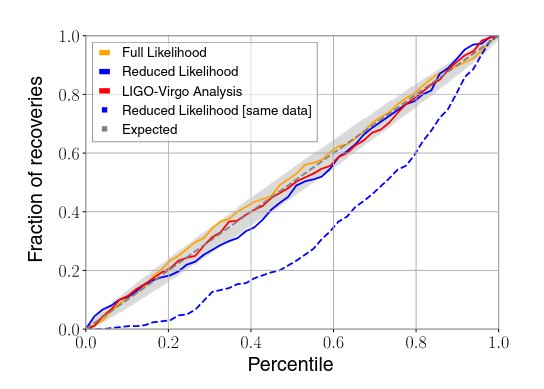
\includegraphics[scale=.45]{fig4.png}
    \caption{Fig 4}
  \end{figure}
\end{frame}

\begin{frame}
  \frametitle{The Result}
  \begin{figure}
    \centering
    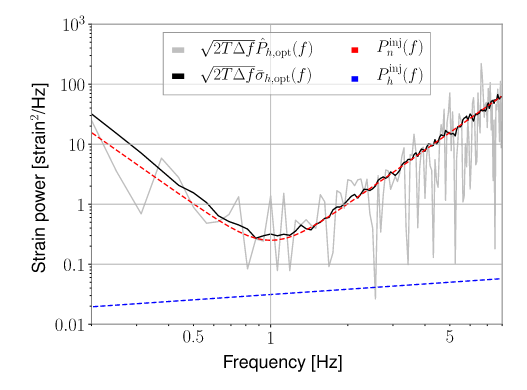
\includegraphics[scale=.3]{fig5top.png}
    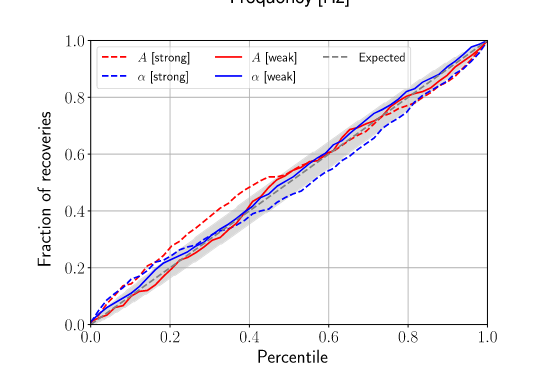
\includegraphics[scale=.3]{fig5bot.png}
  \end{figure}
\end{frame}

\begin{frame}
  \frametitle{Critical Analysis}
  \begin{itemize}
  \item Admirable exposition overall; the distance between computational steps was sensible, and the typesetting clear and consistent.
  \item One illustrative example is sufficient.
    If results really supersede each other, just go through the pain to derive the general one, then deduce the simplifications,
    and explain that the simplifications came first (Research-order, not textbook-order! No one reads derivations unless they have reason to).
  \item Multiple overlapping histograms are hard to read.
    Use cubic-spline interpolations, and if you're concerned about misinterpretation, indicate the histogram midpoints; it's easier on the reader.
  \end{itemize}
\end{frame}

\begin{frame}
  \frametitle{Appendix: Captions}
  \begin{figure}
    \centering
    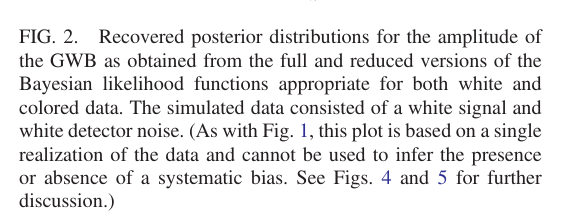
\includegraphics[scale=.3]{fig2txt.png}
    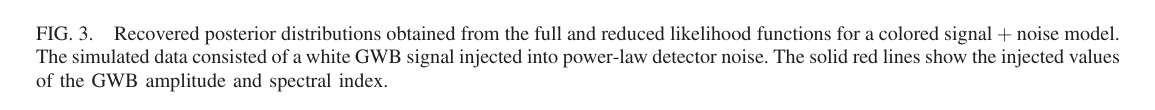
\includegraphics[scale=.28]{fig3txt.png}
    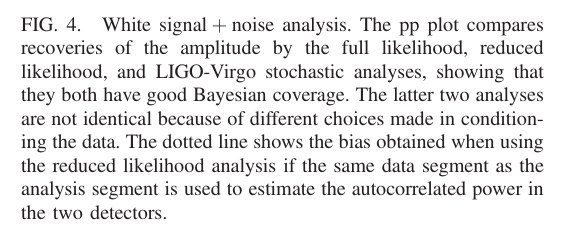
\includegraphics[scale=.3]{fig4txt.png}
  \end{figure}
\end{frame}

\begin{frame}
  \frametitle{Appendix: Captions}
  \begin{figure}
    \centering
    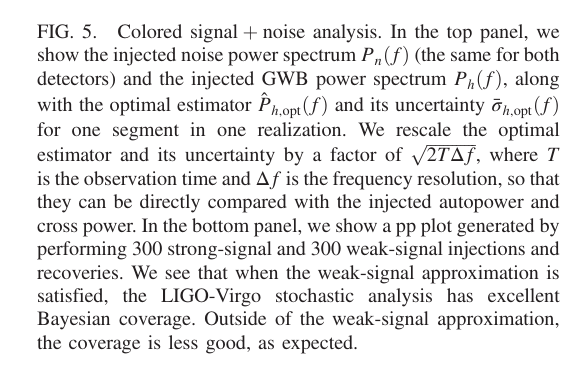
\includegraphics[scale=.3]{fig5txt.png}

  \end{figure}
\end{frame}

\begin{frame}
  \frametitle{Appendix: Equations}
  \begin{figure}
    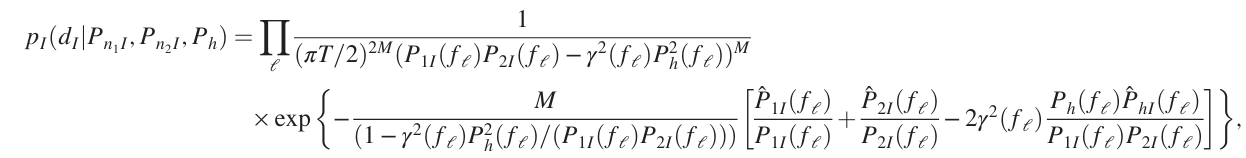
\includegraphics[scale=.25]{full.png}
    \caption{Full, colored, moving-signal likelihood}
    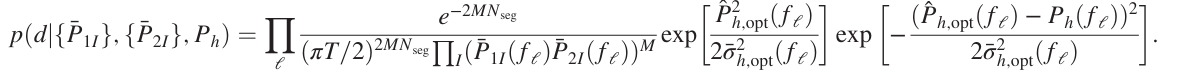
\includegraphics[scale=.25]{reduced.png}
    \caption{Reduced, colored, moving-signal likelihood}
    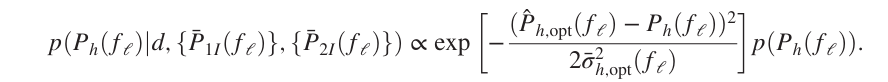
\includegraphics[scale=.25]{propto.png}
    \caption{Reduced likelihood is sufficient}
  \end{figure}
\end{frame}
\end{document}
%%% Local Variables:
%%% mode: latex
%%% TeX-master: t
%%% End:
